\subsection{Sudoku Dataset}
\label{section:rank angle sudoku complete}

Figures~\ref{fig:rank sudoku complete} and~\ref{fig:angle sudoku complete} capture the evolution of the effective rank and average angle of all heads. Most of them follow the separation dynamics on the hypersphere where tokens tend to be near-orthogonal, corroborating our design goal of attention energy. 
% \begin{figure}[htbp]
%     \centering
%     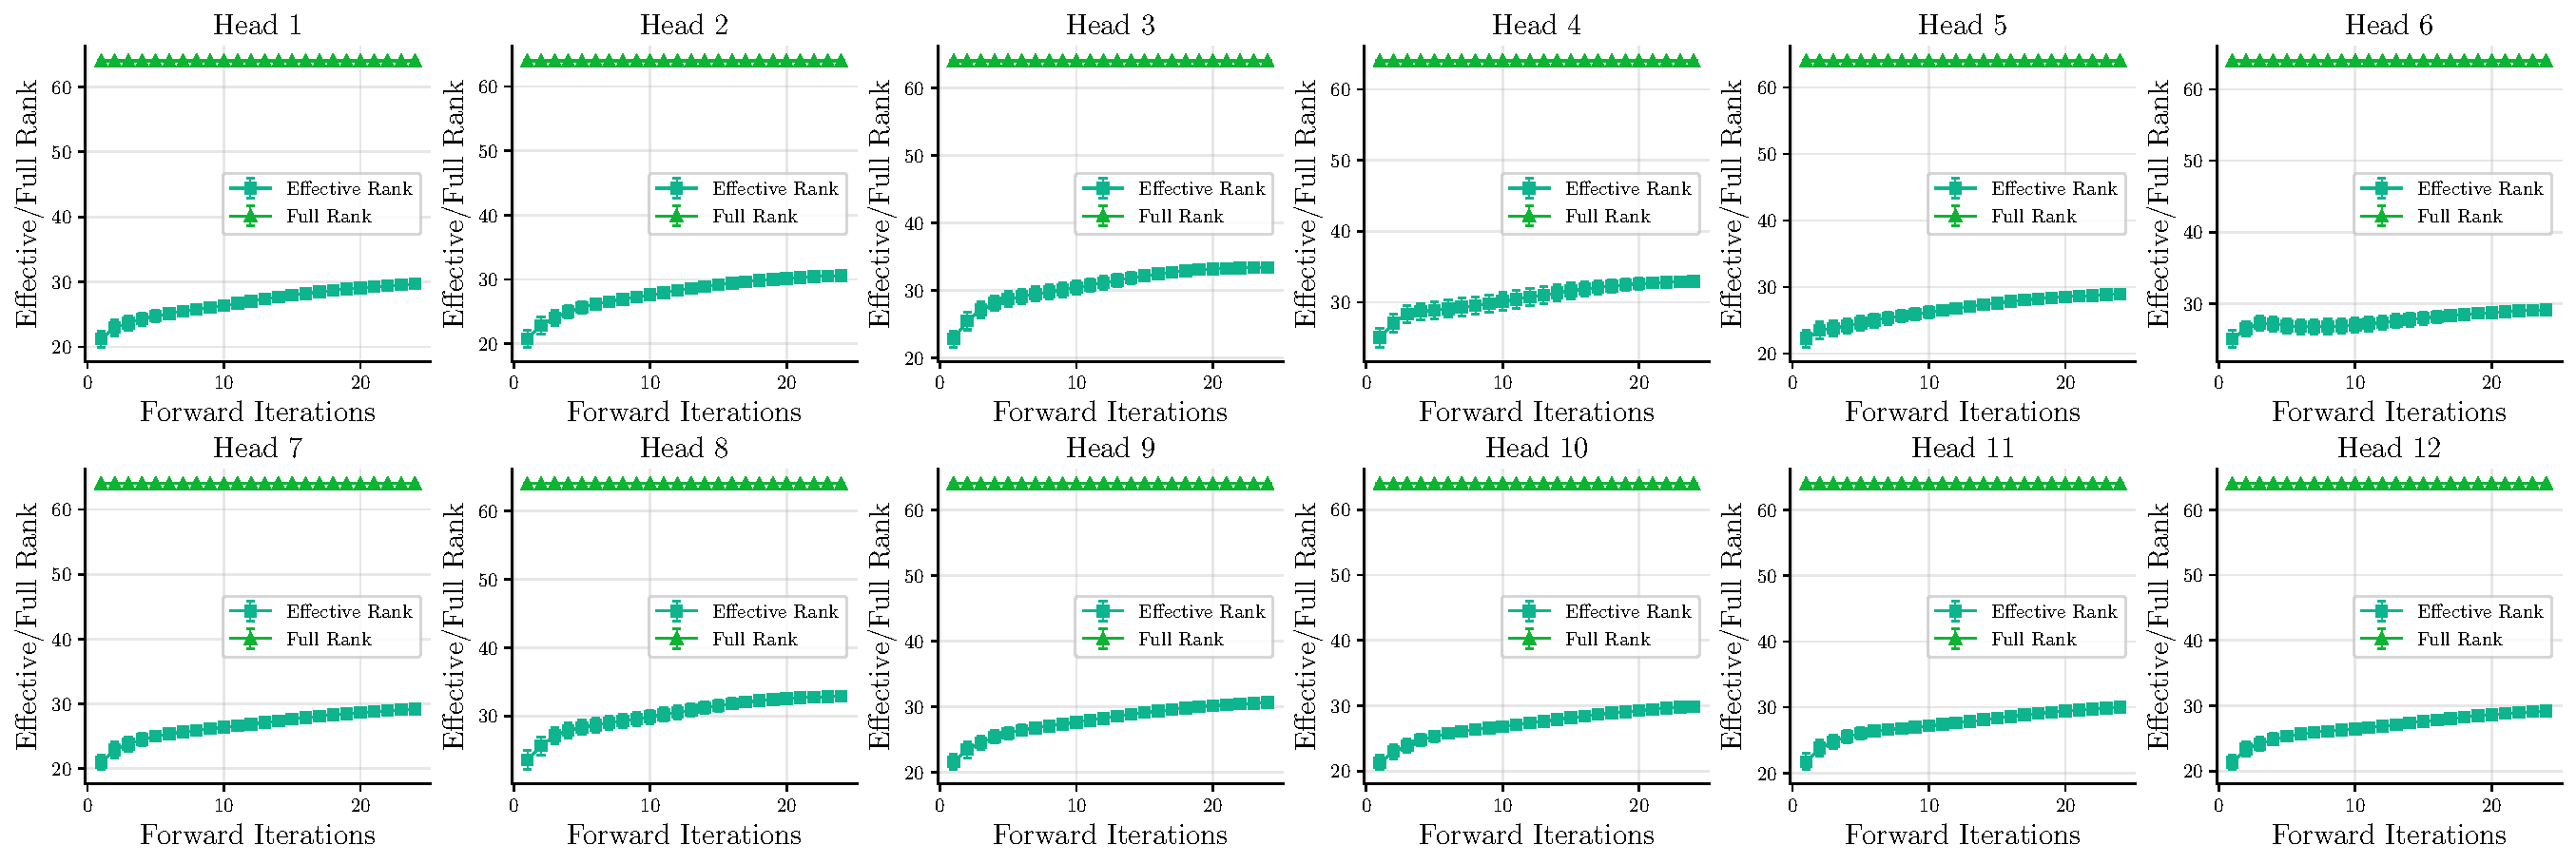
\includegraphics[width=\linewidth]{figures/rank_sudoku.pdf}
%     \caption{The effective rank of tokens projected to each subspace. Results are from the test set of Sudoku dataset \citep{palm2018recurrent}.}
%     \label{fig:rank sudoku complete}
% \end{figure}
% \begin{figure}[htbp]
%     \centering
%     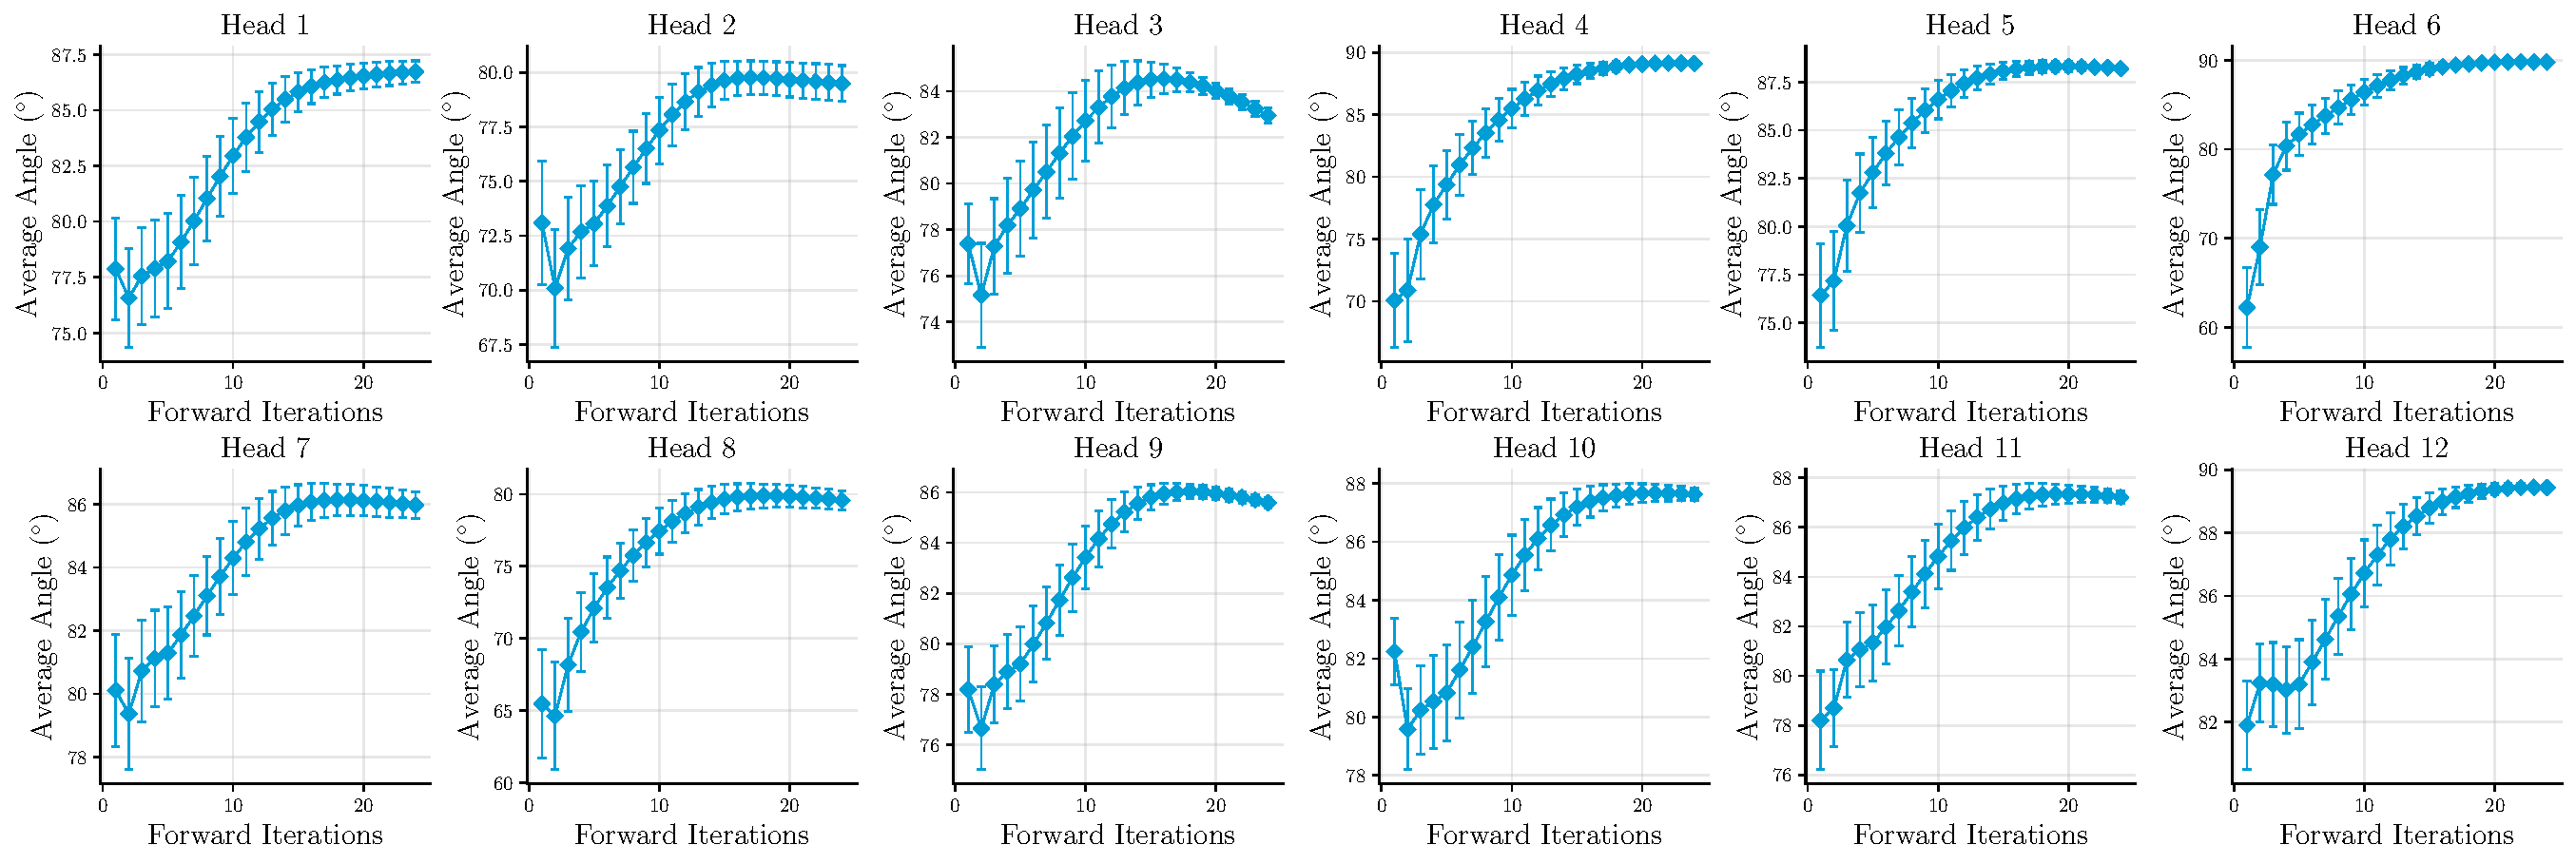
\includegraphics[width=\linewidth]{figures/angle_sudoku.pdf}
%     \caption{The average angle of tokens projected to each subspace. Results are from the test set of Sudoku dataset \citep{palm2018recurrent}.}
%     \label{fig:angle sudoku complete}
% \end{figure}
\begin{figure}[htbp]
  \centering
  % --- Subfigure 1 ---
  \begin{subfigure}[b]{\textwidth} % Control width here (e.g. 0.8 or 0.9)
    \centering
    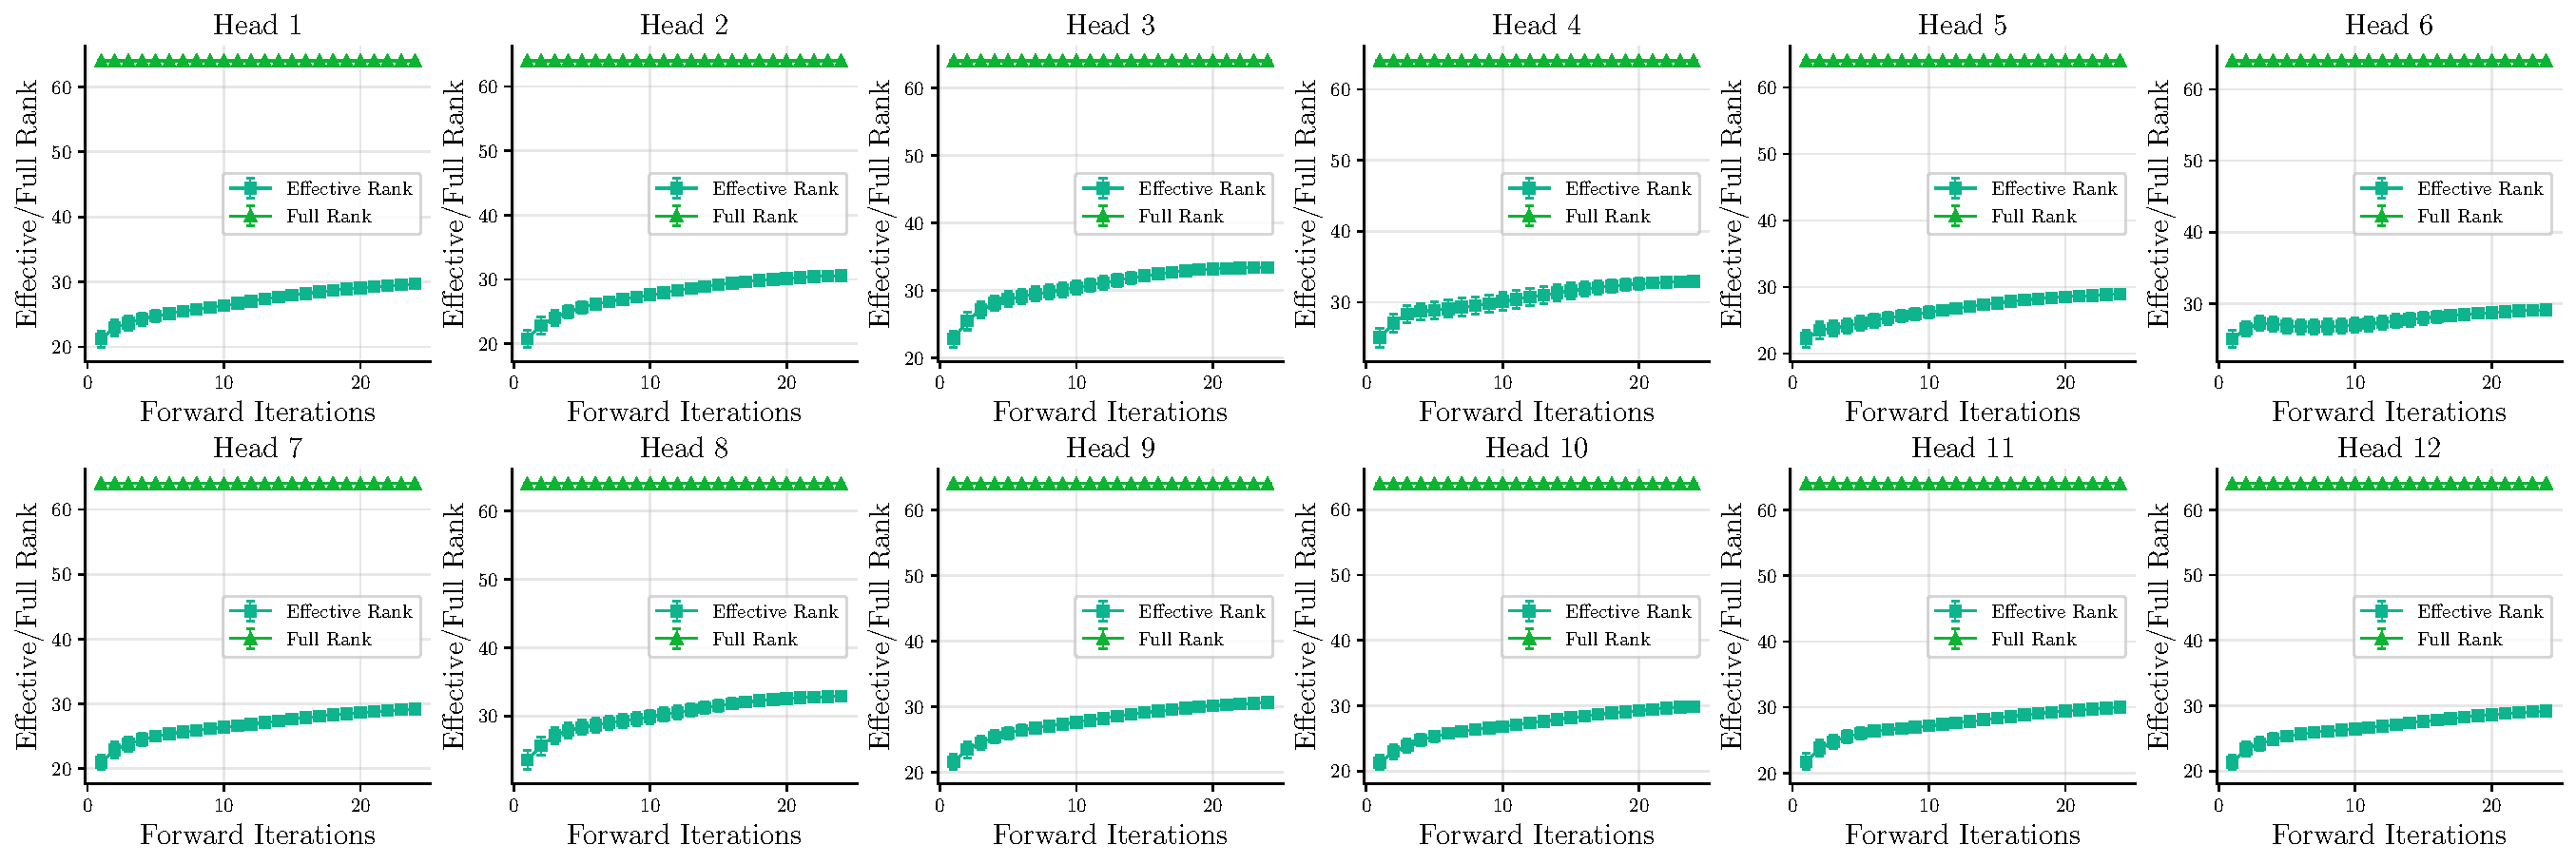
\includegraphics[width=\linewidth]{figures/rank_sudoku.pdf}
    \caption{Effective and full rank.}
    \label{fig:rank sudoku complete}
  \end{subfigure}
  
  \vspace{1em} % Space between the two rows
  
  % --- Subfigure 2 ---
  \begin{subfigure}[b]{\textwidth}
    \centering
    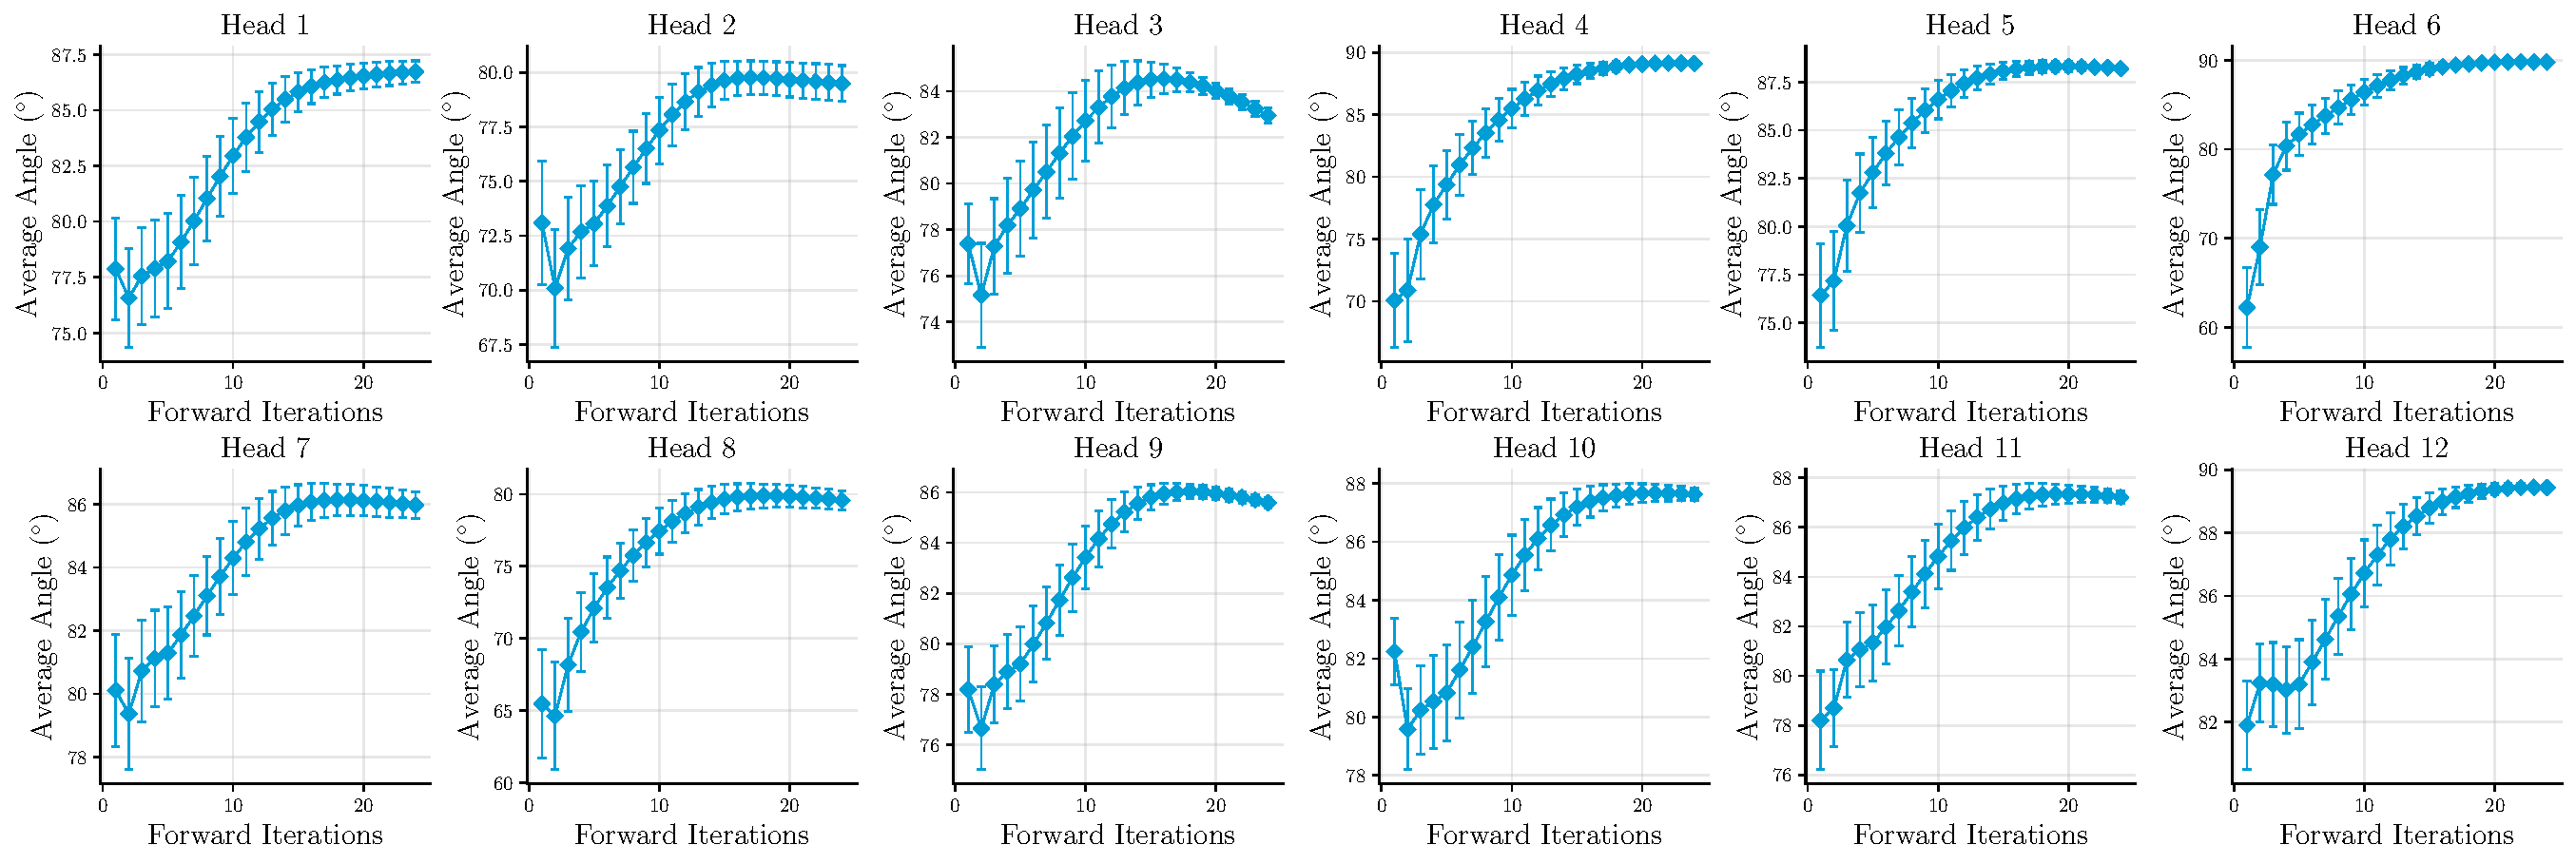
\includegraphics[width=\linewidth]{figures/angle_sudoku.pdf}
    \caption{Average angle.}
    \label{fig:angle sudoku complete}
  \end{subfigure}
  
  \caption{Geometric analysis on Sudoku. The effective rank (a) and average angle (b) of tokens projected to each subspace on the test set \citep{palm2018recurrent}.}
  \label{fig:rank angle sudoku complete}
\end{figure}
%%%%%%%%%%%%%%%%%%%%%%%%%%%%%%%%%%%%%%%%%%%%%%%%%%%%%%%%%%%%%%%%%%%%%%%%%%%%%%%
%%%%%%%%%%%%%%%%%%%%%%%%%%%%%%%%%%%%%%%%%%%%%%%%%%%%%%%%%%%%%%%%%%%%%%%%%%%%%%%
\subsection{CIFAR-10 Dataset}
\label{section:rank angle cifar10 complete}
The full results on CIFAR-10 also possess similar trends to those on the Sudoku dataset, as shown in Figures~\ref{fig:rank cifar10 complete} and~\ref{fig:angle cifar10 complete}.

% \begin{figure}[htbp]
%     \centering
%     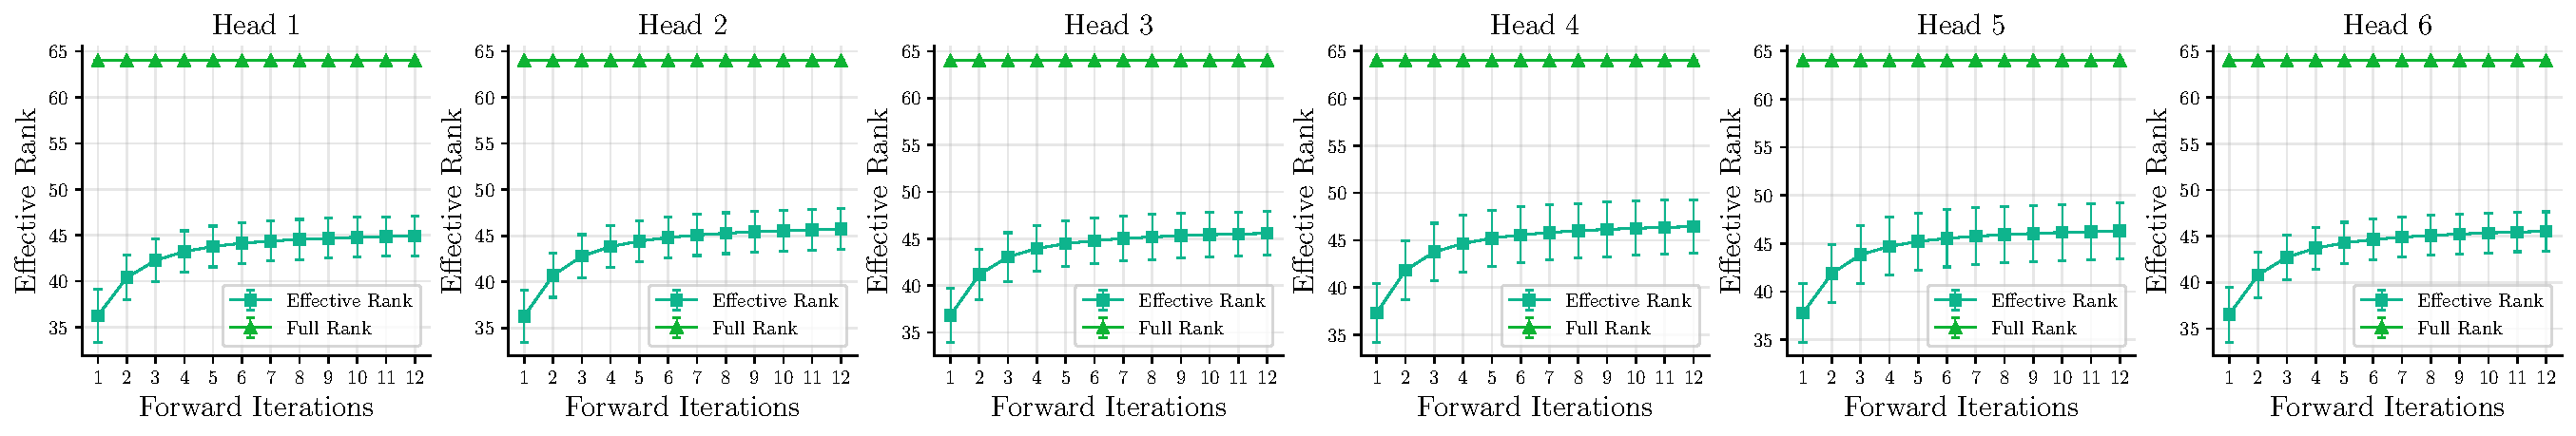
\includegraphics[width=\linewidth]{figures/rank-v2.pdf}
%     \caption{The effective rank of tokens projected to each subspace. Results are from CIFAR-10 validation set.}
%     \label{fig:rank cifar10 complete}
% \end{figure}
% \begin{figure}[htbp]
%     \centering
%     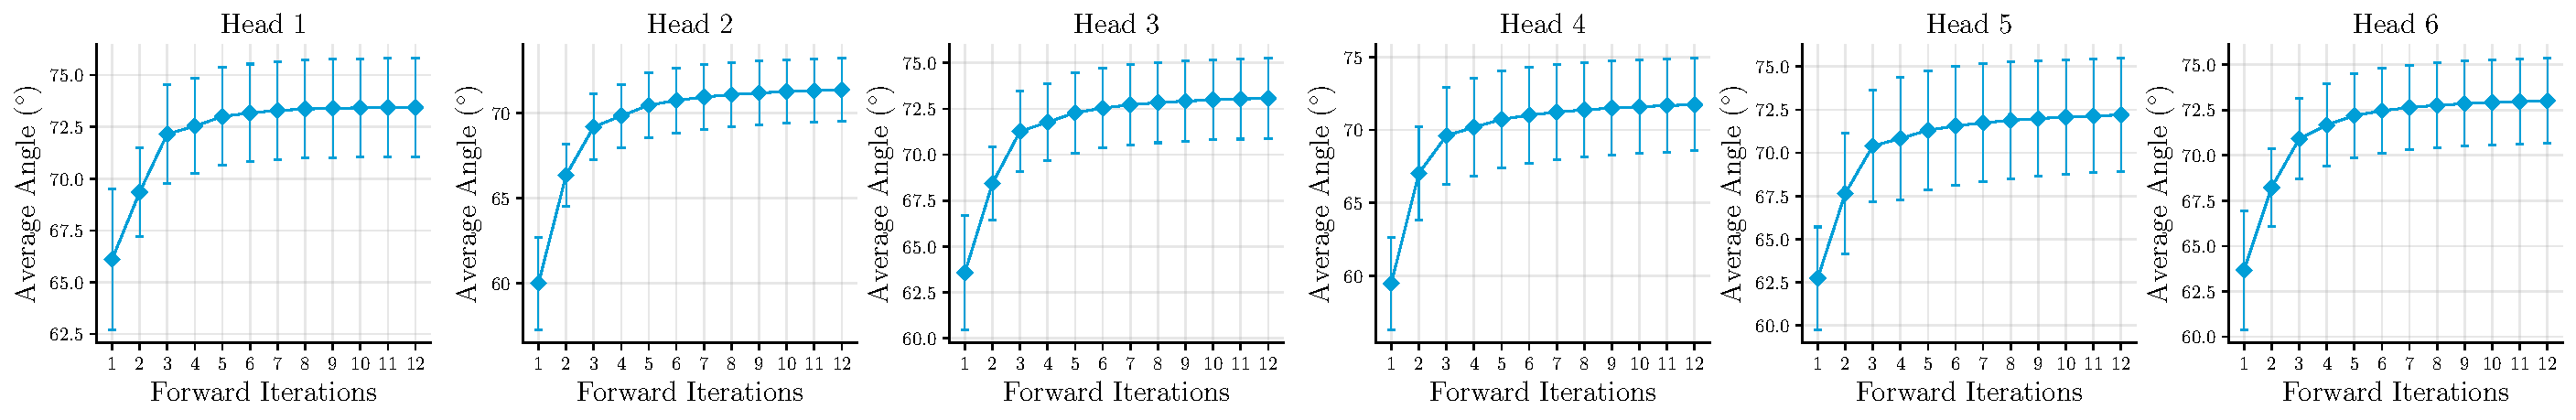
\includegraphics[width=\linewidth]{figures/angle-v2.pdf}
%     \caption{The average angle of tokens projected to each subspace. Results are from CIFAR-10 validation set.}
%     \label{fig:angle cifar10 complete}
% \end{figure}

\begin{figure}[htbp]
  \centering
  % --- Subfigure 1 ---
  \begin{subfigure}[b]{\textwidth} % Control width here (e.g. 0.8 or 0.9)
    \centering
    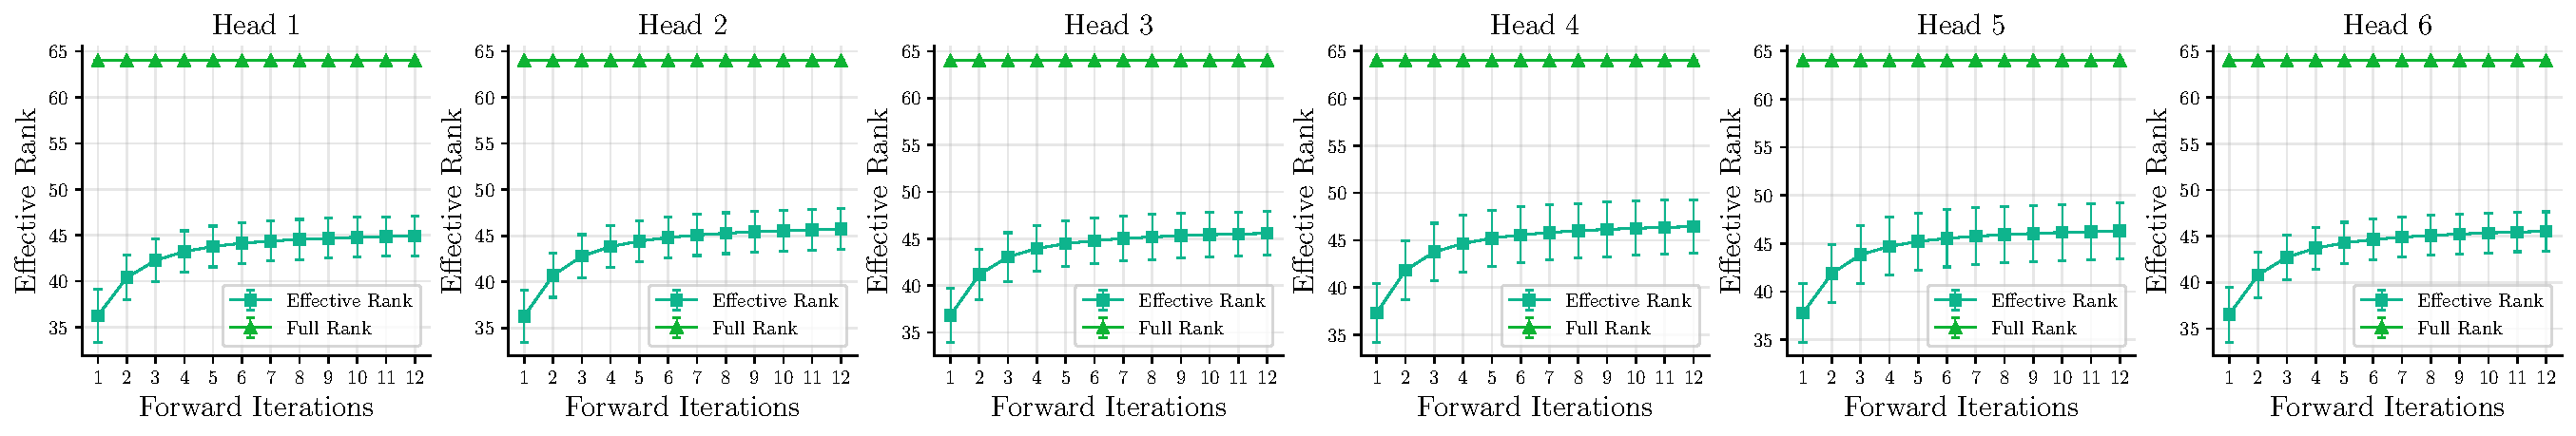
\includegraphics[width=\linewidth]{figures/rank-v2.pdf}
    \caption{Effective and full rank.}
    \label{fig:rank cifar10 complete}
  \end{subfigure}
  
  \vspace{1em} % Space between the two rows
  
  % --- Subfigure 2 ---
  \begin{subfigure}[b]{\textwidth}
    \centering
    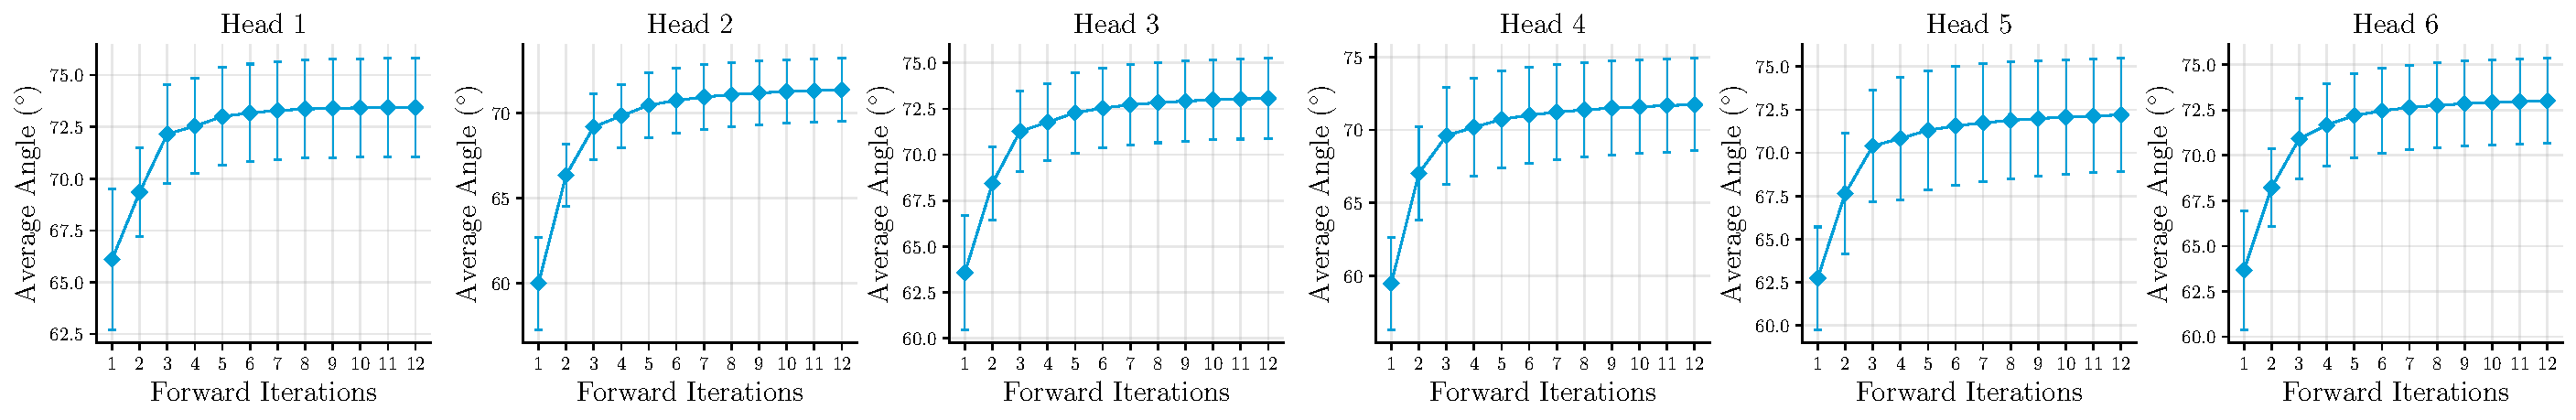
\includegraphics[width=\linewidth]{figures/angle-v2.pdf}
    \caption{Average angle.}
    \label{fig:angle cifar10 complete}
  \end{subfigure}
  
  \caption{Geometric analysis on CIFAR-10. The effective rank (a) and average angle (b) of tokens projected to each subspace on the test set \citep{palm2018recurrent}.}
  \label{fig:rank angle cifar10 complete}
\end{figure}


\subsection{Comparisons with Transformer with Shared Query, Key, and Value Matrix}

A notable connection between \textsc{Hyper-SET} and vanilla Transformer lies in the shared query (Q), key (K), and value (V) projection matrix, which has been studied recently \citep{kowsher-etal-2025-self}. To verify whether \textsc{Hyper-SET} captures essential Transformer behaviors, we adapt vanilla Transformer to have shared QKV projections and measure its effective rank and average angle among projected tokens. Furthermore, we also include comparisons with \textsc{Hyper-SET} that adopts fixed step sizes set as 0.1 to evaluate the necessity of learned ones.

As shown in Figures~\ref{fig:rank shared QKV cifar10 complete} and~\ref{fig:angle shared QKV cifar10 complete}, both \textsc{Hyper-SET} and its fixed-step variant exhibit increasing token separation across subspaces, confirming the emergence of distributional uniformity and the benefit of learned step sizes. This dynamics is also mirrored in shared QKV Transformer, which cross-validates our insights on distributional uniformity in subspaces, suggesting the promise of this parameter-sharing design. In contrast, modifying the shared Transformer to reverse the update direction of attention—similar to the design in~\Eqref{eq:8}—leads to a decline in both rank and angle, highlighting a breakdown in uniformity. This contrast emphasizes that \textsc{Hyper-SET} is not a heuristic tweak of vanilla Transformer but a principled architecture.

% \begin{figure}[htbp]
%     \centering
%     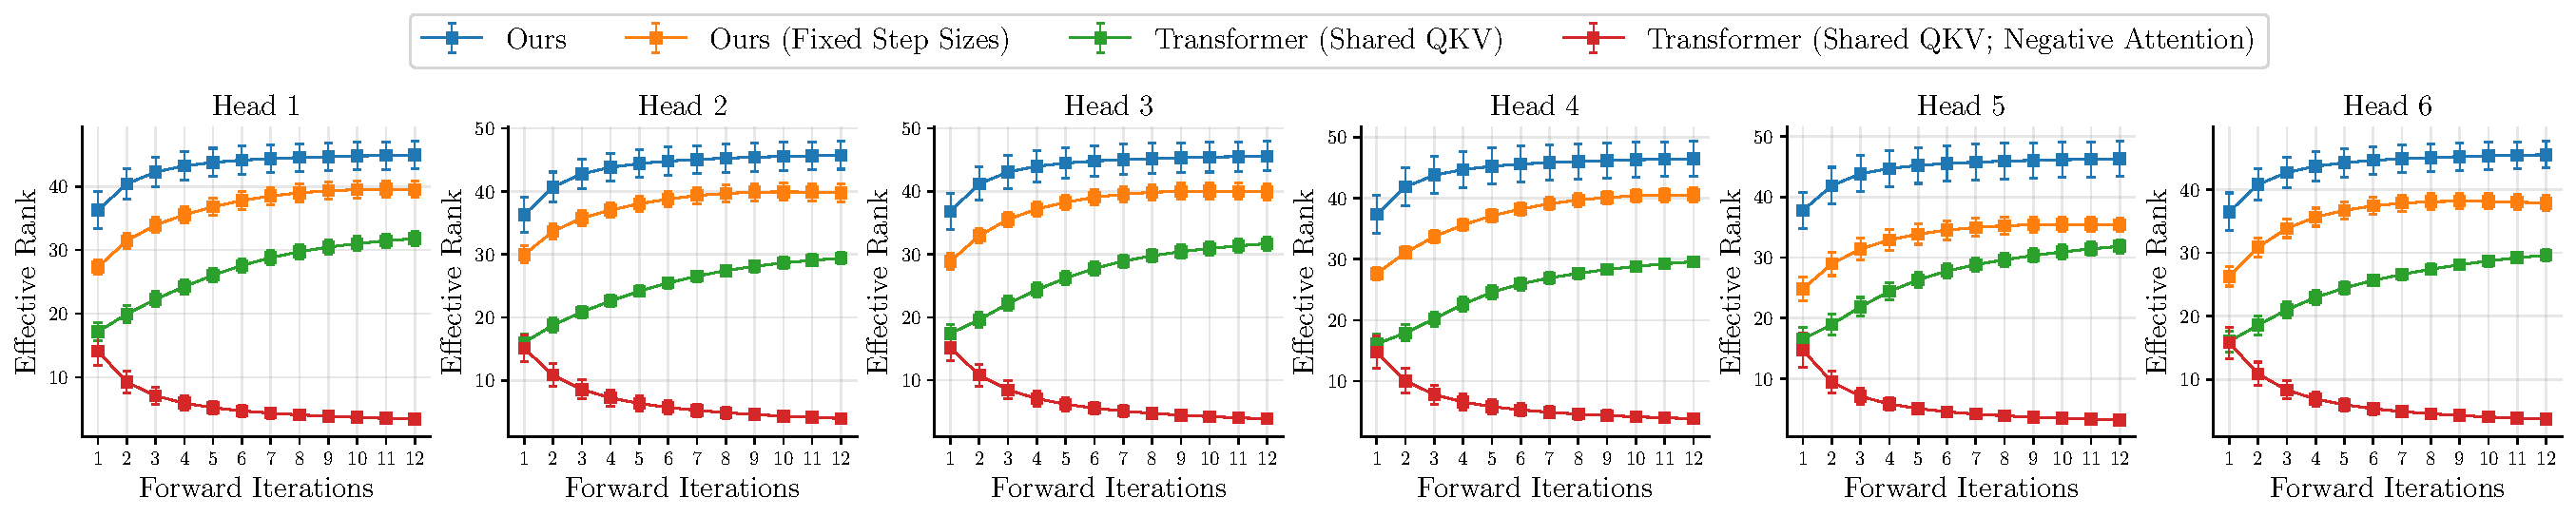
\includegraphics[width=\linewidth]{figures/rank_shared_QKV.pdf}
%     \caption{Comparisons of the effective rank at each subspace with fixed step sizes, Transformer with shared query/key/value matrix, and reverting the update sign before its attention. Results are from CIFAR-10 validation set.}
%     \label{fig:rank shared QKV cifar10 complete}
% \end{figure}
% \begin{figure}[htbp]
%     \centering
%     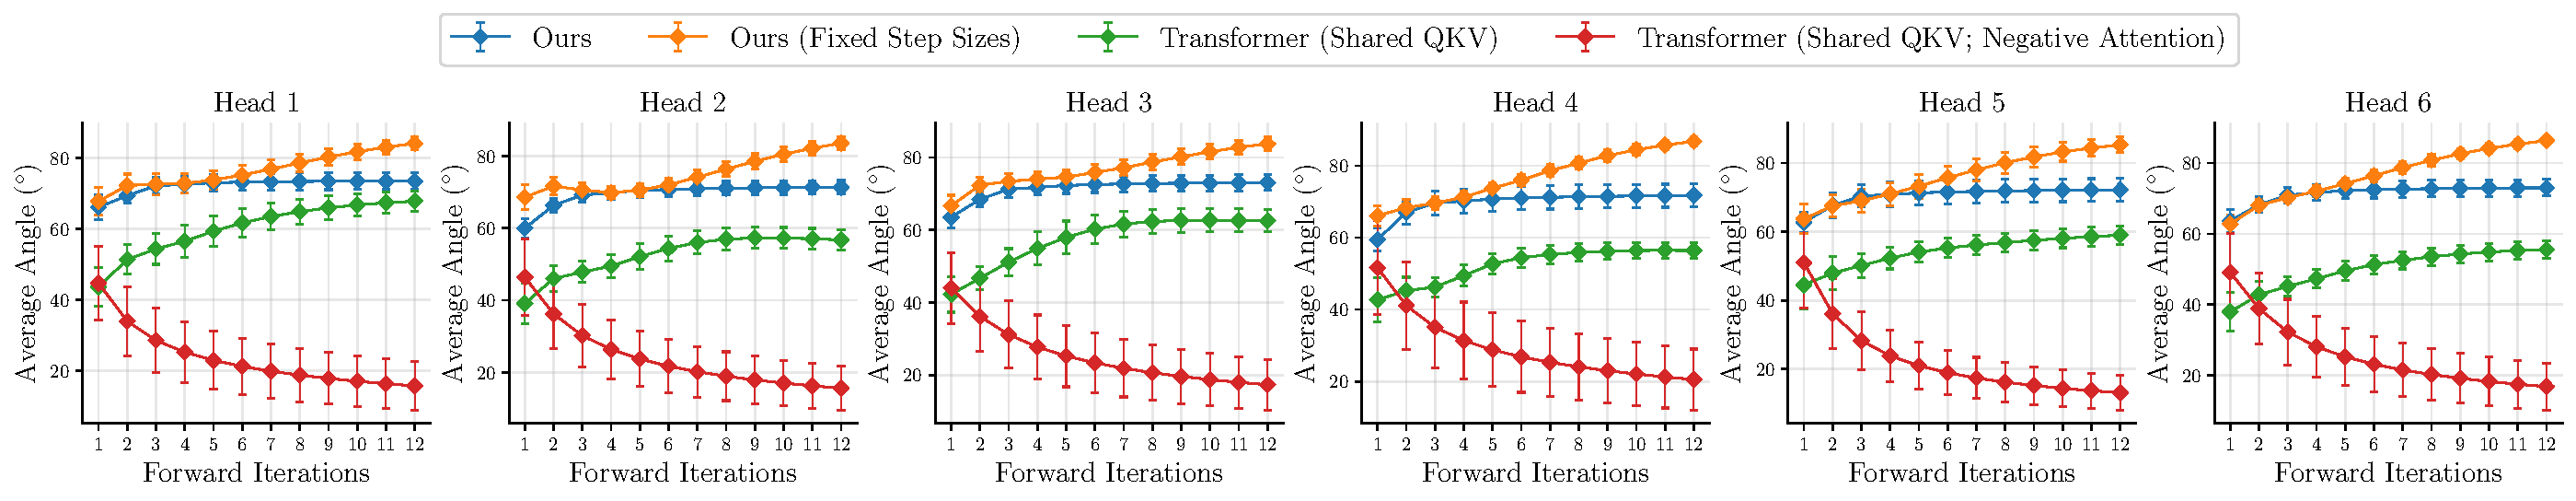
\includegraphics[width=\linewidth]{figures/angle_shared_QKV.pdf}
%     \caption{Comparisons of the average angle at each subspace with fixed step sizes, Transformer with shared query/key/value matrix, and reverting the update sign before its attention. Results are from CIFAR-10 validation set.}
%     \label{fig:angle shared QKV cifar10 complete}
% \end{figure}
\begin{figure}[htbp]
    \centering
    % --- Subfigure 1: Rank ---
    \begin{subfigure}[b]{0.95\linewidth}
        \centering
        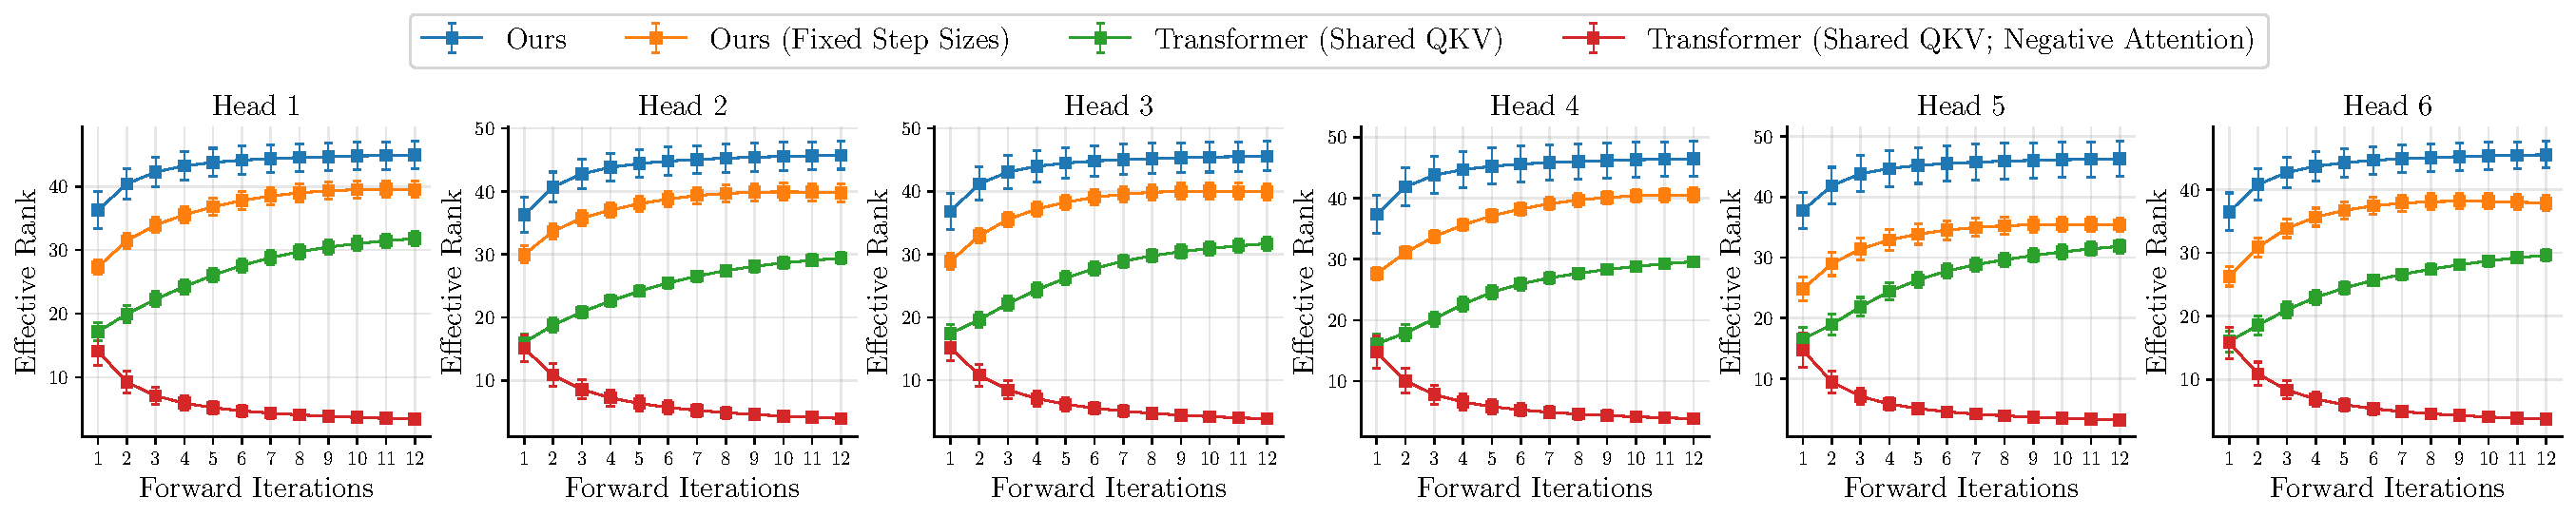
\includegraphics[width=\linewidth]{figures/rank_shared_QKV.pdf}
        \caption{Effective rank.}
        \label{fig:rank shared QKV cifar10 complete}
    \end{subfigure}
    
    \vspace{1em} % Vertical spacing between the two plots
    
    % --- Subfigure 2: Angle ---
    \begin{subfigure}[b]{0.95\linewidth}
        \centering
        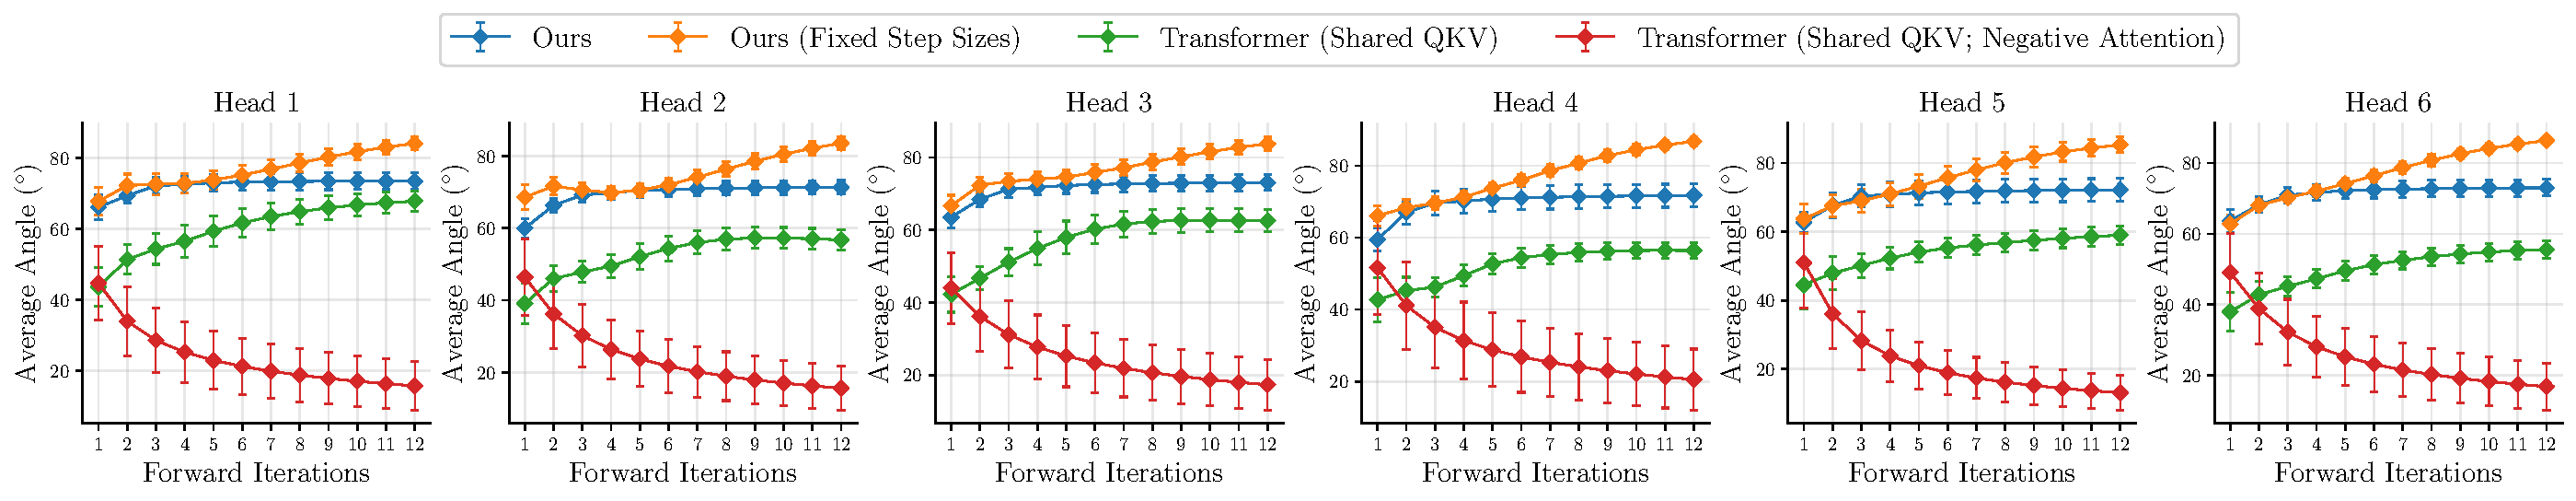
\includegraphics[width=\linewidth]{figures/angle_shared_QKV.pdf}
        \caption{Average Angle.}
        \label{fig:angle shared QKV cifar10 complete}
    \end{subfigure}
    
    \caption{Impact of weight sharing and update rules. This layer-wise evolution of effective rank (\emph{Top}) and average angle (\emph{Bottom}) on the CIFAR-10 validation set verifies that our architecture and the variant using fixed step sizes share a similar functional role with Transformer with shared Query/Key/Value (QKV) matrices.}
    \label{fig:rank angle shared QKV cifar10 complete}
\end{figure}